\documentclass[a4paper, 10pt, dvipdfmx]{jlreq}

\usepackage{amsmath,amsfonts,amssymb}
\usepackage{bm}
\usepackage{mathtools}
\usepackage{siunitx}
\usepackage[dvipdfmx]{graphicx}
\usepackage[dvipdfmx]{color}
\usepackage[dvipdfmx, colorlinks=true, allcolors=blue]{hyperref}
\usepackage{listings, jlisting}
\usepackage{tikz}
\usepackage{physics}
\usepackage{url}

\Urlmuskip=0mu plus 10mu
\allowdisplaybreaks[4]
\frenchspacing
\definecolor{OliveGreen}{rgb}{0.0,0.6,0.0}
\definecolor{Orenge}{rgb}{0.89,0.55,0}
\definecolor{SkyBlue}{rgb}{0.28, 0.28, 0.95}
\lstset{
  language={c++},
  basicstyle={\ttfamily},
  identifierstyle={\small},
  ndkeywordstyle={\small},
  frame=single,
  breaklines=true,
  numbers=left,
  xrightmargin=0zw,
  xleftmargin=3zw,
  numberstyle={\scriptsize},
  lineskip=-0.9ex,
  keywordstyle={\small\bfseries\color{SkyBlue}},  
  commentstyle={\color{OliveGreen}}, 
  stringstyle={\small\ttfamily\color{Orenge}}    
}

\begin{document}

\title{2015年度 大問3}
\author{hari64boli64 (hari64boli64@gmail.com)}
\date{\today}
\maketitle

\section{問題}

\begin{align*}
  \begin{cases}
    \dv{x}{t}=x(t)-y(t)-x(t)(x(t)^2+y(t)^2)+\frac{x(t)y(t)}{\sqrt{x(t)^2+y(t)^2}} \\
    \dv{y}{t}=x(t)+y(t)-y(t)(x(t)^2+y(t)^2)-\frac{x(t)^2}{\sqrt{x(t)^2+y(t)^2}}   \\
  \end{cases}
\end{align*}

\section{解答}

\subsection*{(1)}

\begin{align*}
  \begin{cases}
    \dv{r}{t}=r-r^3 \\
    \dv{\theta}{t}=1-\cos{\theta}
  \end{cases}
\end{align*}

\subsection*{(2)}

\begin{align*}
              & \begin{cases}
    \dv{r}{t}=r-r^3               \\
    \dv{\theta}{t}=1-\cos{\theta} \\
  \end{cases} \\
  \Rightarrow & \begin{cases}
    \int \frac{1}{r-r^3} dr=\int dt                  \\
    \int \frac{1}{1-\cos{\theta}}\dv{\theta}=\int dt \\
  \end{cases} \\
  \Rightarrow & \begin{cases}
    r=\sqrt{\frac{1}{\qty(\frac{1}{r_0^2}-1)e^{-2t}+1}}              \\
    \theta=2\arctan{\frac{1}{-t+\frac{1}{\tan{\frac{\theta_0}{2}}}}} \\
  \end{cases}
\end{align*}

前者は部分分数分解、後者は三角関数の半角公式を用いて解いた。

見えやすいのでこのままにしたが、もう少し簡略化すべき。

\subsection*{(3),(4)}

\begin{figure}[htbp]
  \begin{center}
    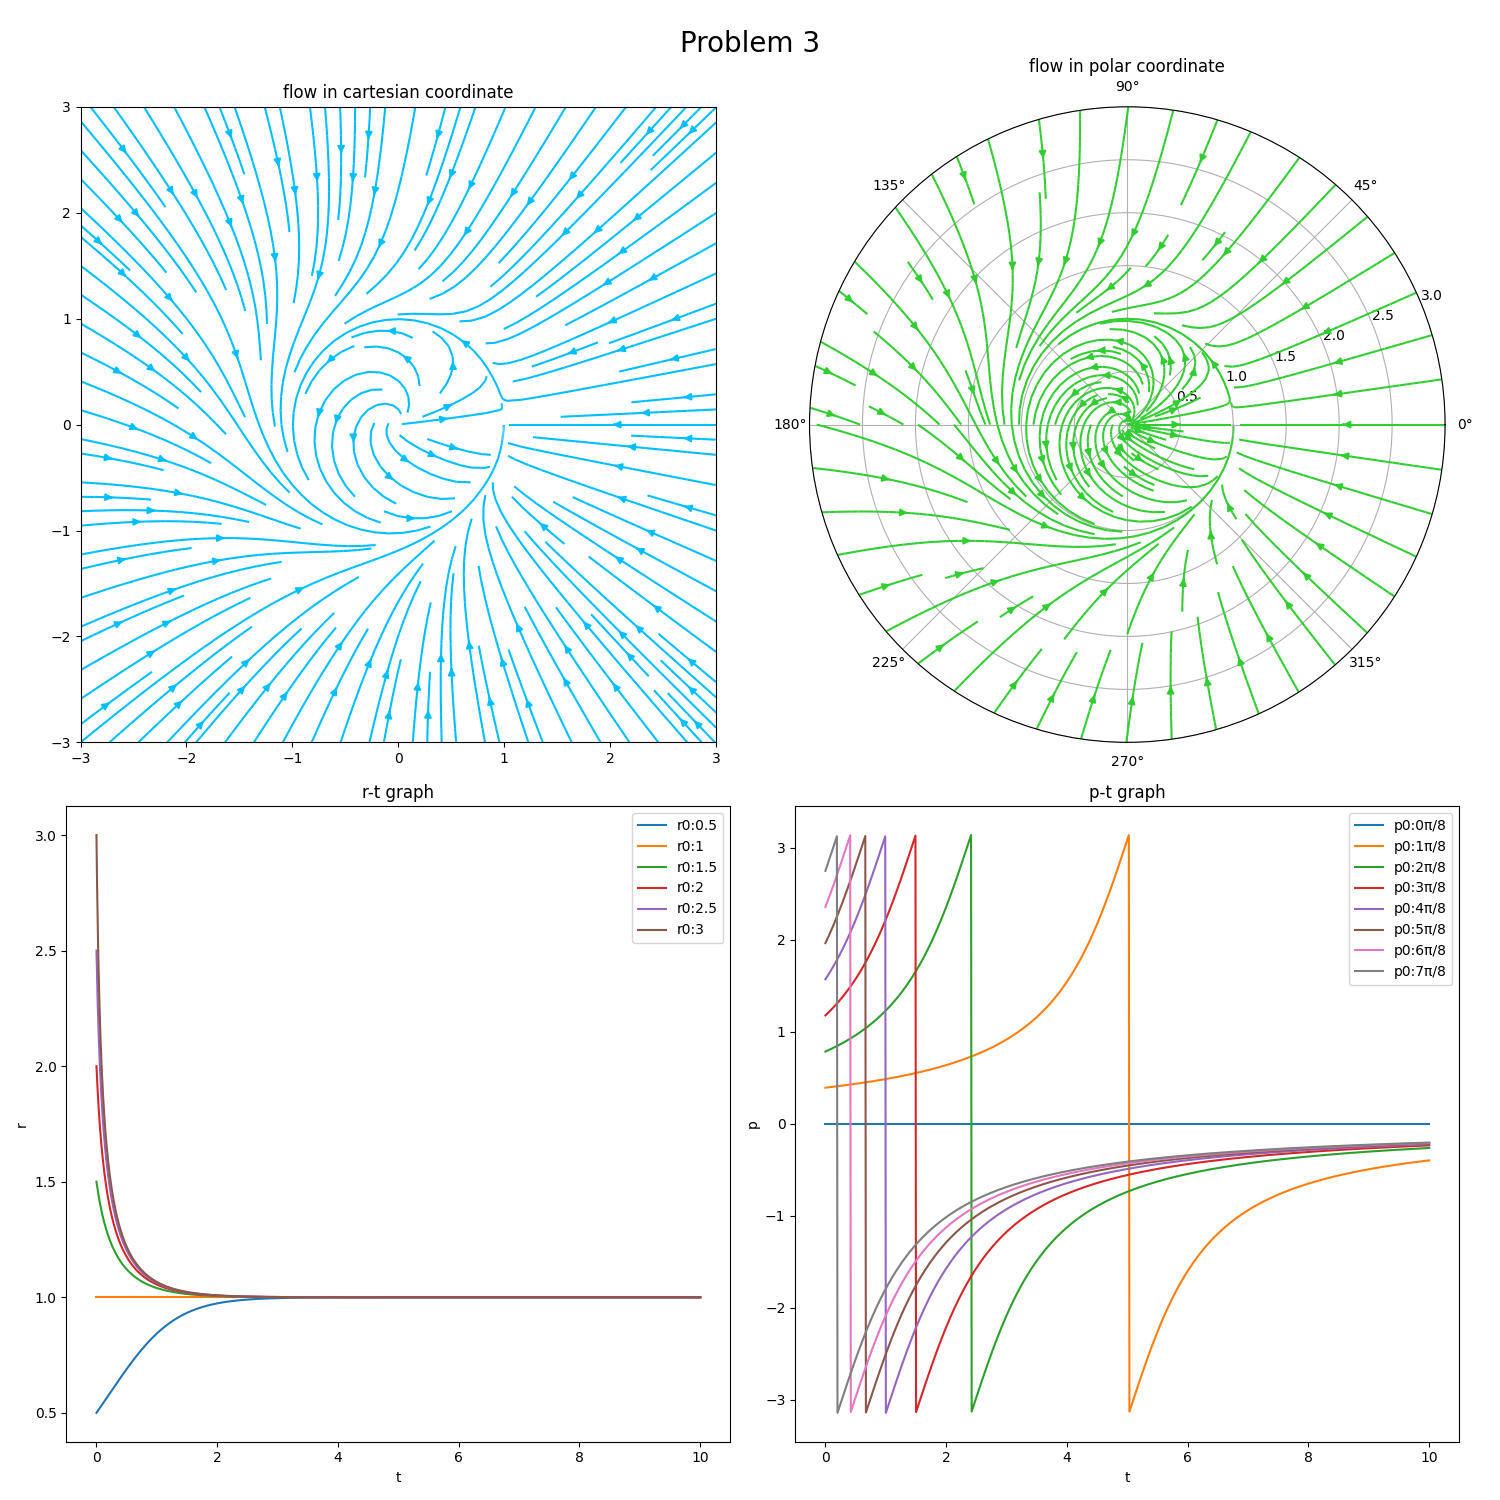
\includegraphics[height=150mm]{3.png}
    \caption{visualizations}
    \label{img:vis}
  \end{center}
\end{figure}

$p$は$\theta$を意味する。角度のグラフに関しては、Pythonのarctanの仕様のため不連続点が生じているが、本来はシグモイド的なグラフを描くべきだろう。

特に、$r_0=1.0, \theta_0=0.0$のとき、これは安定固定点となる。

\section{知識}

忘れている公式類があまりに多いので、全て記しておく。

\subsection{三角関数}

\subsubsection{二倍角の公式}

\begin{align*}
  \sin{2x} & =2\sin{x}\cos{x}              \\
  \cos{2x} & =\cos{x}^2-\sin{x}^2          \\
           & =2\cos^2{x}-1                 \\
           & =1-2\sin^2{x}                 \\
  \tan{2x} & =\frac{2\tan{x}}{1-\tan{x}^2}
\end{align*}

\subsubsection{二倍角の公式の逆}

\begin{align*}
  \sin^2{x}=\frac{1-\cos{2x}}{2} \\
  \cos^2{x}=\frac{1+\cos{2x}}{2}
\end{align*}

\subsubsection{三倍角の公式}

\begin{align*}
  \sin{3x} & =3\sin{x}-4\sin^3{x} \\
  \cos{3x} & =4\cos^3{x}-3\cos{x}
\end{align*}

\subsubsection{三倍角の公式の逆}

\begin{align*}
  \sin^3{x}=\frac{3\sin{x}-\sin{3x}}{4} \\
  \cos^3{x}=\frac{3\cos{x}+\cos{3x}}{4}
\end{align*}

\subsubsection{和積の公式}

\begin{align*}
  \sin{x}+\sin{y}=2\sin{\frac{x+y}{2}}\cos{\frac{x-y}{2}} \\
  \sin{x}-\sin{y}=2\cos{\frac{x+y}{2}}\sin{\frac{x-y}{2}} \\
  \cos{x}+\cos{y}=2\cos{\frac{x+y}{2}}\cos{\frac{x-y}{2}} \\
  \cos{x}-\cos{y}=-2\sin{\frac{x+y}{2}}\sin{\frac{x-y}{2}}
\end{align*}

\subsubsection{積和の逆}

\begin{align*}
  \sin{x}\cos{y} & =\frac{1}{2}\qty(\sin{(x+y)}+\sin{(x-y)})  \\
  \cos{x}\sin{y} & =\frac{1}{2}\qty(\sin{(x+y)}-\sin{(x-y)})  \\
  \cos{x}\cos{y} & =\frac{1}{2}\qty(\cos{(x+y)}+\cos{(x-y)})  \\
  \sin{x}\sin{y} & =-\frac{1}{2}\qty(\cos{(x+y)}-\cos{(x-y)})
\end{align*}

\subsection{積分}

\subsubsection{$1\pm\cos{x}$}

\begin{align*}
  \int \frac{1}{1+\cos{x}}dx & = \int \frac{1}{2\cos^2{\frac{x}{2}}} dx \\
                             & = \tan{\frac{x}{2}}+C
\end{align*}

\subsubsection{$1\pm\sin{x}$}

\begin{align*}
  \int \frac{1}{1+\sin{x}}dx & = \int \frac{1}{1+\cos{(\frac{\pi}{2}-x)}} dx            \\
                             & = \int \frac{1}{2\cos^2{(\frac{\pi}{4}-\frac{x}{2})}} dx \\
                             & = -\tan{(\frac{\pi}{4}-\frac{x}{2})}+C
\end{align*}

これらは、分母分子に$1\mp\cos{x}$や$1\mp\sin{x}$をかける事でも求められる。

また、最悪の場合、$\tan{\frac{x}{2}}$を$t$と置くと、

\begin{align*}
  \sin{x}=\frac{2t}{1+t^2} \\
  \cos{x}=\frac{1-t^2}{1+t^2}
\end{align*}

となって、助かることがある。

\subsubsection{$x^2+a^2$}

本題とは関連がないが、忘れていたので書いておく。

\begin{align*}
  \int \frac{1}{x^2+a^2} dx & = \int \frac{1}{a^2}\cos{^2\theta} \frac{a}{\cos^2{\theta}}d\theta \quad (x=a\tan{\theta}) \\
                            & = \frac{1}{a}\arctan{\frac{x}{a}}+C                                                        \\
\end{align*}

\subsubsection{$\sqrt{x^2+a^2}$}

本題とは関連がないが、忘れていたので書いておく。

受験の月で最高難度とされているやつ。

\begin{align*}
  \int \frac{1}{\sqrt{x^2+1}} dx & = \int \frac{1}{t} dt \quad (t=x+\sqrt{x^2+1}) \\
                                 & = \log{\qty(x+\sqrt{x^2+1})}+C                 \\
\end{align*}


\section{おまけ}

\href{3.py}{3.py}がビジュアライズ用のコードである。

\lstinputlisting[caption=visualizer,label=code:visualizer,language=Python]{3.py}

\begin{thebibliography}{9}
  \bibitem{site:1}
  matplotlib.“matplotlib.pyplot.streamplot”.2020年1月5日.\url{https://matplotlib.org/3.1.1/api/_as_gen/matplotlib.pyplot.streamplot.html}
  \bibitem{site:2}
  受験の月."高校数学3 積分法(基本計算パターン)".\url{https://examist.jp/category/mathematics/integration/}
\end{thebibliography}

\end{document}
